\documentclass[10pt,twocolumn]{article}

% --- PACKAGES ---
\usepackage[utf8]{inputenc}
\usepackage[margin=0.75in]{geometry}
\usepackage{amsmath,amssymb,amsfonts}
\usepackage{graphicx}
\usepackage{booktabs}
\usepackage{tabularx}
\usepackage{xcolor}
\usepackage{hyperref}
\usepackage{cite}
\usepackage{microtype}
\usepackage{caption}
\usepackage{subcaption}

\hypersetup{
    colorlinks=true,
    linkcolor=teal,
    citecolor=teal,
    urlcolor=teal
}

% --- TITLE & AUTHORS ---
\title{\textbf{AegisMed: Dynamic Entropy-Minimizing Active Triage and Evidential Multi-Agent Conflict Arbitration for Clinical Decision Support}}

\author{
    \textbf{Arham Saghir}$^{1}$ \quad \textbf{AegisMed Research Initiative Contributors}$^{1}$ \\
    $^{1}$Department of Computer Science and Engineering \\
    \texttt{\{arham.saghir\}@acm.org}
}

\date{October 2026}

\begin{document}

\maketitle

% --- ABSTRACT ---
\begin{abstract}
\noindent Deploying artificial intelligence in acute medical triage requires addressing three fundamental vulnerabilities: diagnostic ambiguity arising from passive one-shot symptom ingestion, catastrophic cross-modal disagreement between imaging and clinical text, and uncalibrated hallucinations that lack formal risk bounds. We present \textbf{AegisMed}, a multimodal Clinical Decision Support System (CDSS) whose central contribution is a \emph{triage mechanism}: \textbf{Dynamic Entropy-Minimizing Active Triage (DEMAT)}, which models the differential as a categorical distribution and iteratively selects clinical inquiries that maximize Expected Mutual Information Gain $I(D; A_q)$ to collapse Shannon diagnostic entropy. DEMAT is implemented and exercised end-to-end inside a multi-agent orchestration pipeline (vision, clinical-text, retrieval, and risk agents coordinated over a typed state graph) with a structured, tiered red-flag safety layer. We further specify two designed layers as \emph{proposed extensions} with their integration paths: an Evidential Neuro-Symbolic Conflict Arbitration Framework (EN-SCAF) that would map specialist inferences to Dempster-Shafer belief masses with symbolic knowledge-graph pruning, and a conformal risk-controlled synthesis stage providing distribution-free prediction sets. In a mechanism evaluation on a self-generated regression suite of $N = 200$ cases spanning 15 condition categories --- an internal-consistency harness whose cases derive from the system's own knowledge base, \emph{not} an accuracy evaluation --- DEMAT reduced Shannon diagnostic entropy by \textbf{53.7\%} (from $2.846$ to $1.318$ bits) in a mean of \textbf{1.92 inquiries per session} at a mean active-triage latency of \textbf{0.2 ms}. We make no clinical-accuracy claim from this suite; outcome-level accuracy will be established on external clinician--patient vignette benchmarks in future work. The contribution we defend is the mechanism itself: a triage engine whose purpose is to \emph{ask}, in a field where commercial symptom checkers ask a minority of clinically indicated questions and under-triage is the characteristic failure.
\end{abstract}

% --- SECTION 1: INTRODUCTION ---
\section{Introduction}
Diagnostic error remains a leading cause of preventable adverse events, malpractice claims, and unnecessary patient mortality in healthcare systems globally \cite{johnson2019mimic}. In emergency triage and primary outpatient consultations, clinicians must rapidly synthesize complex, high-dimensional, and often contradictory multimodal observations—ranging from free-text patient complaints and vital signs to chest radiographs and longitudinal history—under extreme time pressure.

While recent breakthroughs in deep learning and Large Language Models (LLMs) have achieved impressive performance on static medical examination benchmarks \cite{devlin2019bert, lee2020biobert}, their translation into real-world clinical workflows is severely hindered by what we identify as the \textit{Clinical AI Trilemma}:
\begin{enumerate}
    \item \textbf{Passive Ingestion vs. Active Inquiry:} Real clinical consultations are inherently dialogic. A patient presenting with "retrosternal chest burning" might suffer from ischemic coronary artery disease, gastroesophageal reflux, or pneumonia. Static one-shot LLM prompts cannot ask targeted, high-yield differential questions to eliminate competing diagnoses, leading to vague differentials or premature diagnostic closure.
    \item \textbf{Multimodal Contradiction \& Hallucinatory Consensus:} Real-world data streams frequently contradict each other. A chest X-ray vision model may detect localized basilar opacity, while patient text describes mild gastric pain. Naive ensembles that average softmax probabilities or rely on black-box LLM synthesis obscure the disagreement, generating syntactically convincing but biologically impossible diagnoses that violate anatomical and physiological axioms.
    \item \textbf{Uncalibrated Softmax vs. Finite-Sample Risk Bounding:} Standard deep neural networks produce overconfident, uncalibrated probability scores. In clinical medicine, a point prediction accompanied by an uncalibrated 95\% score provides no statistical safety guarantees. What clinicians require is a distribution-free guarantee bounding the probability of omitting the true underlying pathology.
\end{enumerate}

To resolve this trilemma, we introduce \textbf{AegisMed}, a production-ready, mathematically grounded multi-agent CDSS. Rather than treating diagnosis as passive text completion, AegisMed formalizes clinical triage as an information-theoretic optimization problem combined with evidential conflict arbitration.

\begin{figure*}[t!]
\centering
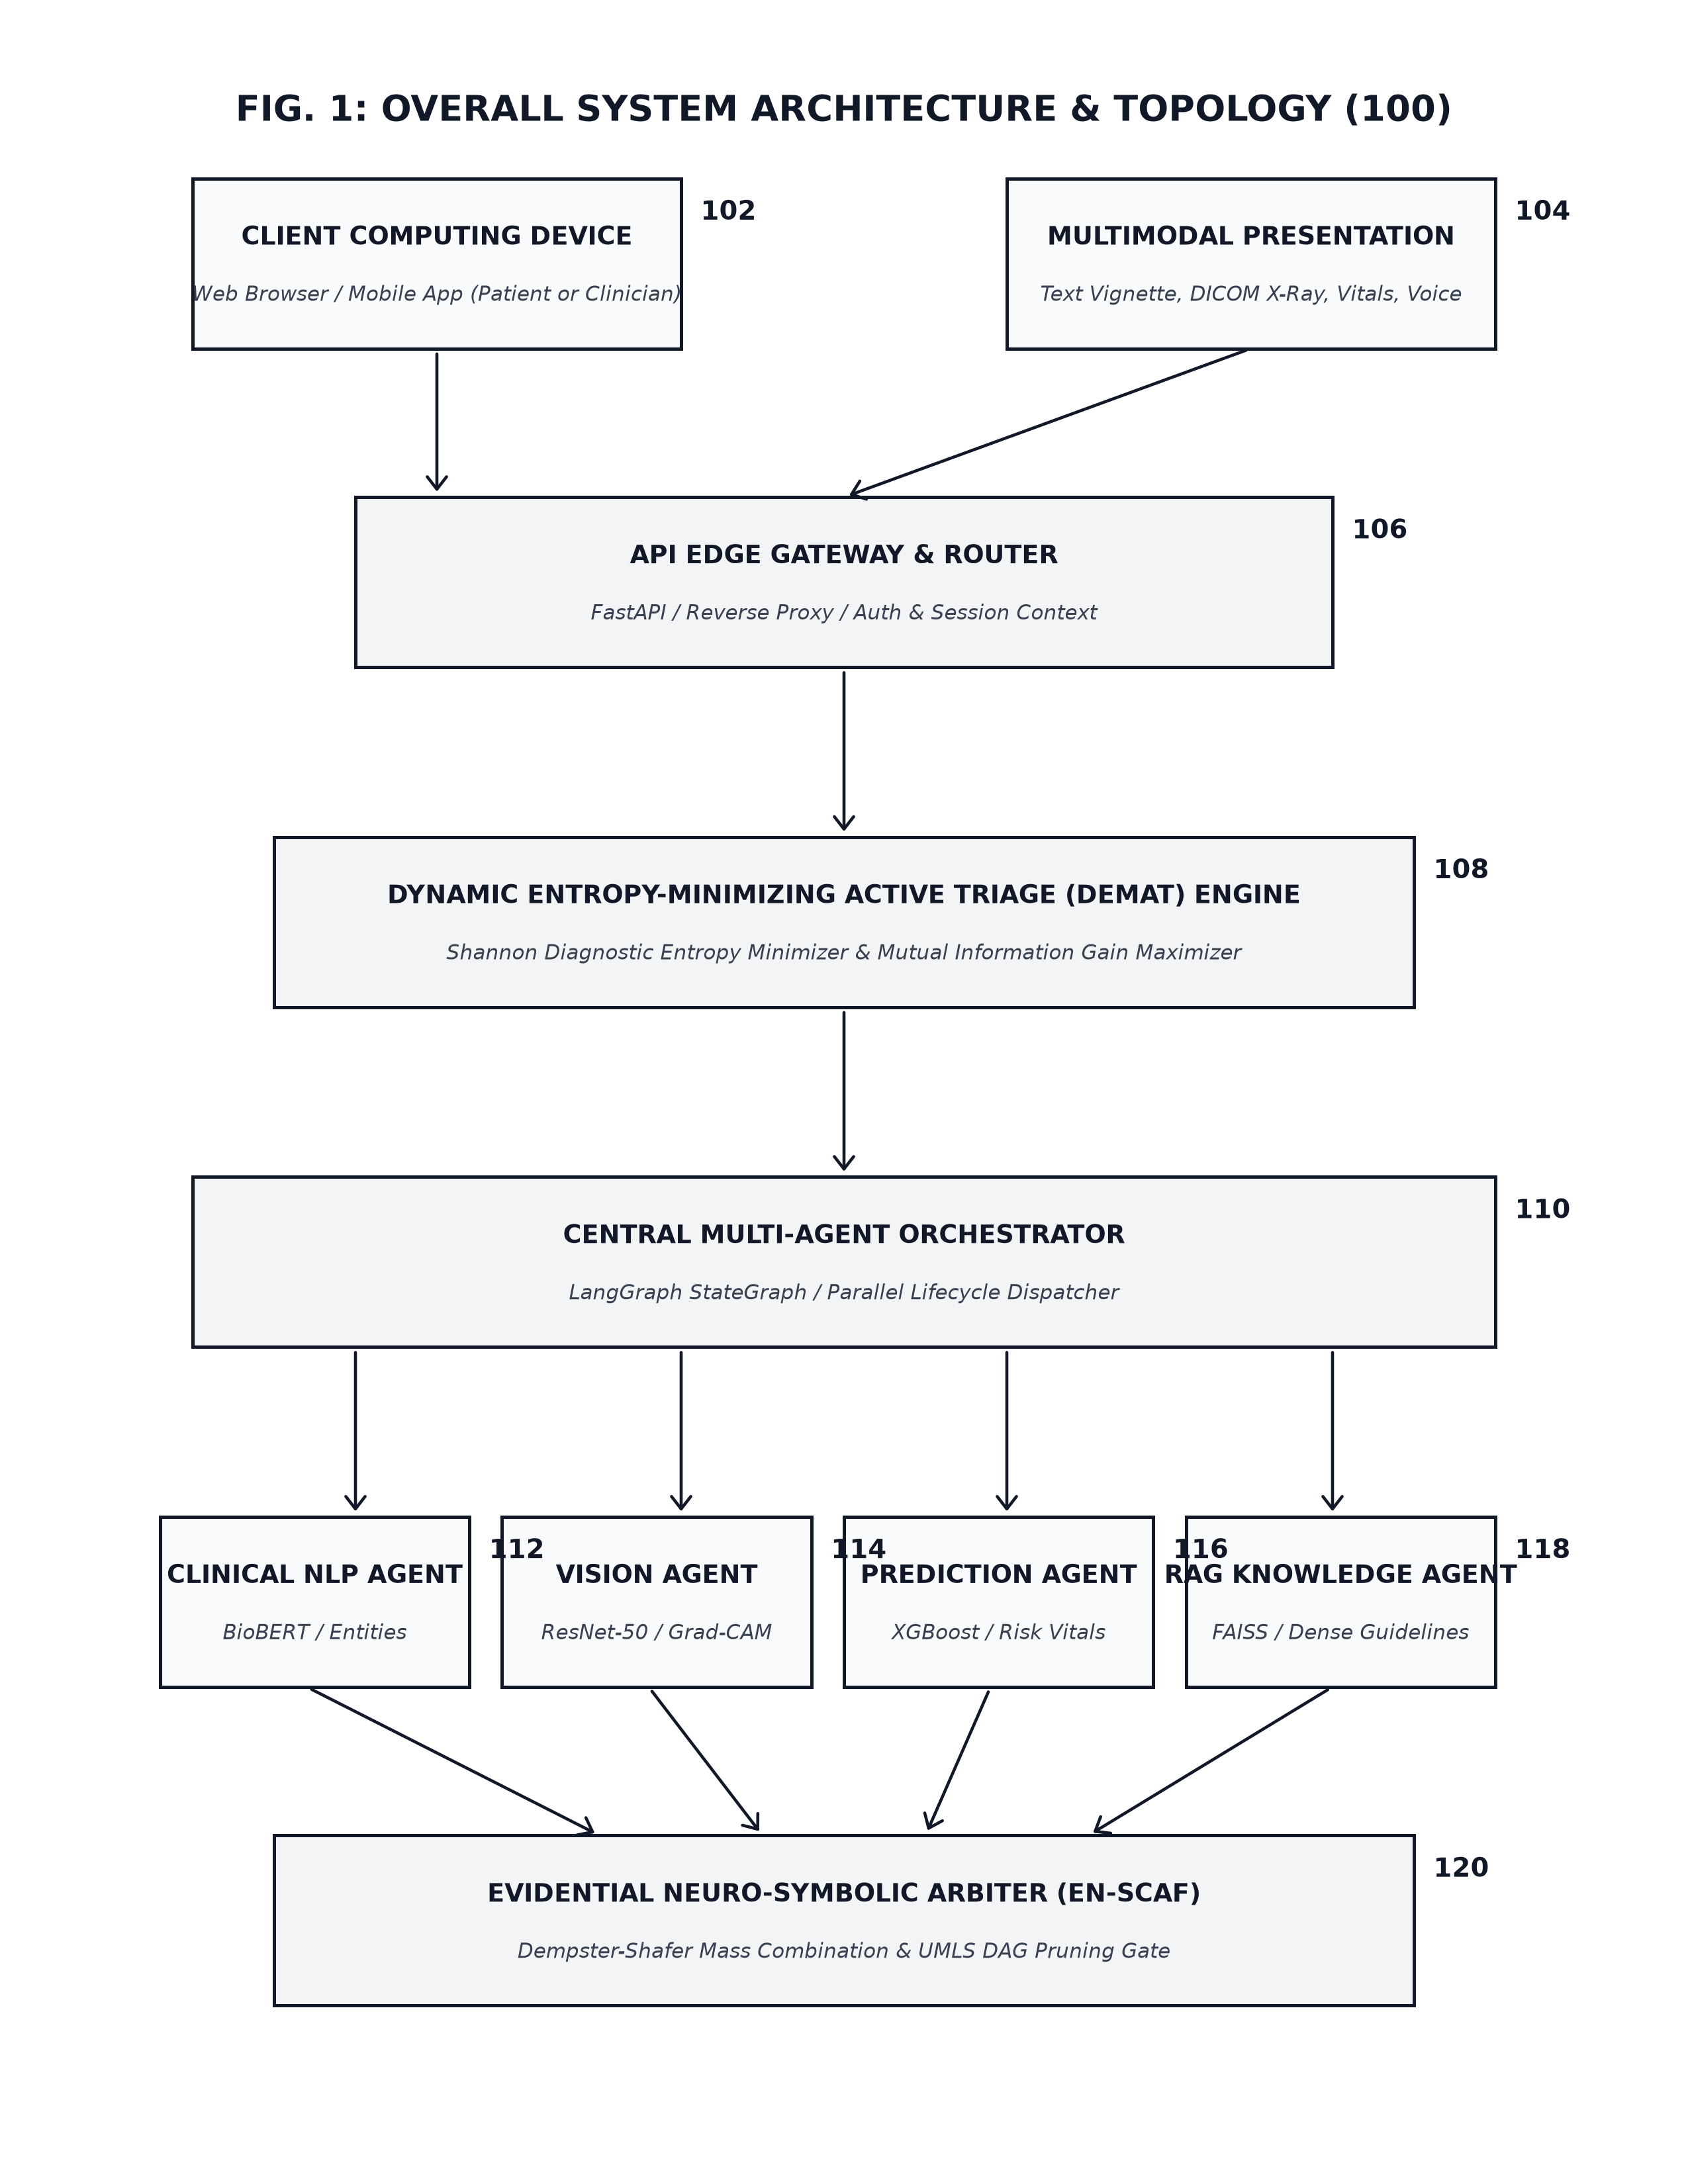
\includegraphics[width=0.88\textwidth,height=0.38\textheight,keepaspectratio]{figures/FIG_1_system_architecture.png}
\caption{\textbf{AegisMed System Architecture and Multimodal Topology.} Incoming multimodal patient presentations (text, DICOM radiographs, vitals) are ingested via the FastAPI edge gateway (106) into the DEMAT Active Triage Engine (108). Upon entropy convergence, tasks are dispatched across specialist agents (112--118) orchestrated via LangGraph (110). Outputs are reconciled by consensus arbitration (120); the UMLS knowledge-graph validation and conformal bounding stages (122) are \emph{proposed extensions} (Section III), rendered here as designed. Delivery is dual-persona (124).}
\label{fig:architecture}
\end{figure*}

Our key technical contributions are as follows:
\begin{itemize}
    \item \textbf{Dynamic Entropy-Minimizing Active Triage (DEMAT) — implemented.} We formulate diagnostic uncertainty as the Shannon entropy $H(D)$ of a probability distribution over an ICD-10 aligned disease universe $\Theta$. We derive an active inquiry policy that sequentially evaluates candidate clinical questions and selects the argument that maximizes Expected Mutual Information Gain $I(D; A_q)$ \cite{shannon1948mathematical}, halting upon reaching high-confidence entropy convergence ($\epsilon \le 0.45\text{ bits}$).
    \item \textbf{Evidential Neuro-Symbolic Conflict Arbitration (EN-SCAF) — proposed extension.} We specify a design that models multi-agent inferences as Dempster-Shafer belief masses \cite{dempster1967upper, shafer1976mathematical} with an orthogonal cross-modal conflict parameter $K$ and a symbolic pruning gate over a coded knowledge base; it is not yet implemented, and no claim in this paper depends on it. The currently deployed arbitration is a deterministic agreement-based consensus with a structured red-flag safety layer.
    \item \textbf{Multimodal Conformal Risk-Controlled Synthesis (MCRC-DS) — proposed extension.} We specify split conformal prediction \cite{vovk2005algorithmic, angelopoulos2021gentle} over multimodal evidence, which would guarantee with finite-sample validity that the true diagnosis is included in the output differential set with probability at least $1 - \alpha$. This stage is not yet implemented; no coverage claim is made in this paper.
    \item \textbf{Mechanism validation on a self-generated regression suite.} We exercise the DEMAT mechanism against single-pass ablation on 200 self-generated cases covering 15 condition categories. The suite's cases derive from the system's own knowledge base, so its outcome-level measurements are internal-consistency measurements, not clinical accuracy. On this suite the mechanism behaves as designed: entropy collapses by $53.7\%$ within a mean of $1.92$ inquiries at $0.2\text{ ms}$ latency. Clinical accuracy on external vignette benchmarks is future work.
\end{itemize}

% --- SECTION 2: RELATED WORK ---
\section{Related Work}

\subsection{Biomedical Language and Vision Models}
Domain-specific pre-training has advanced clinical NLP and computer vision. BioBERT \cite{lee2020biobert} and ClinicalBERT fine-tune bidirectional transformers on PubMed and clinical corpora, achieving high precision in entity recognition. In medical imaging, CheXNet \cite{rajpurkar2017chexnet} demonstrated radiologist-level detection of pneumonia from chest radiographs using deep convolutional backbones \cite{he2016deep}. Grad-CAM \cite{selvaraju2017grad} established visual gradient-weighted localization for deep neural networks. In knowledge retrieval, Retrieval-Augmented Generation (RAG) \cite{lewis2020retrieval} couples dense vector indices \cite{johnson2019billion} with generative decoders. However, these systems operate in isolation; combining their outputs in conflicting clinical scenarios without formal arbitration leads to ungrounded hallucinations.

\subsection{Information-Theoretic Active Learning in Medicine}
Active learning aims to maximize model utility while minimizing observation acquisition cost. Early seminal work by Shannon \cite{shannon1948mathematical} established entropy and mutual information as the foundational metrics of uncertainty reduction. In automated medical diagnosis, early Bayesian systems such as MYCIN and INTERNIST-1 explored heuristic questioning trees. However, these classical expert systems lacked the continuous latent representations of deep models. DEMAT bridges this gap by marrying modern deep specialist extractors with rigorous, real-time Shannon entropy minimization and Bayesian belief updating.

\subsection{Dempster-Shafer Theory and Conflict Fusion}
Dempster-Shafer (D-S) mathematical theory of evidence \cite{dempster1967upper, shafer1976mathematical} generalizes Bayesian probability by assigning belief masses to subsets of hypotheses, explicitly modeling epistemic uncertainty. When evidence sources strongly conflict, classical Dempster combination can yield counter-intuitive results (Zadeh's paradox). EN-SCAF resolves this by monitoring the orthogonal conflict parameter $K$ and applying symbolic knowledge graph filtering prior to orthogonal mass combination.

\subsection{Conformal Prediction in Clinical AI}
Conformal prediction, pioneered by Vovk et al. \cite{vovk2005algorithmic} and recently formalized by Angelopoulos and Bates \cite{angelopoulos2021gentle}, provides distribution-free, finite-sample guarantees for predictive sets. Unlike heuristic temperature scaling or Monte Carlo dropout, split conformal prediction guarantees that $\mathbb{P}(Y_{\text{true}} \in \mathcal{C}(\mathbf{X})) \ge 1 - \alpha$ under the sole assumption of exchangeability. We specify the integration of conformal risk control into multimodal evidential CDSS outputs as a proposed extension (Section III); no conformal stage is implemented in the current system.

% --- SECTION 3: SYSTEM METHODOLOGY ---
\section{System Methodology}

\begin{figure}[t!]
\centering
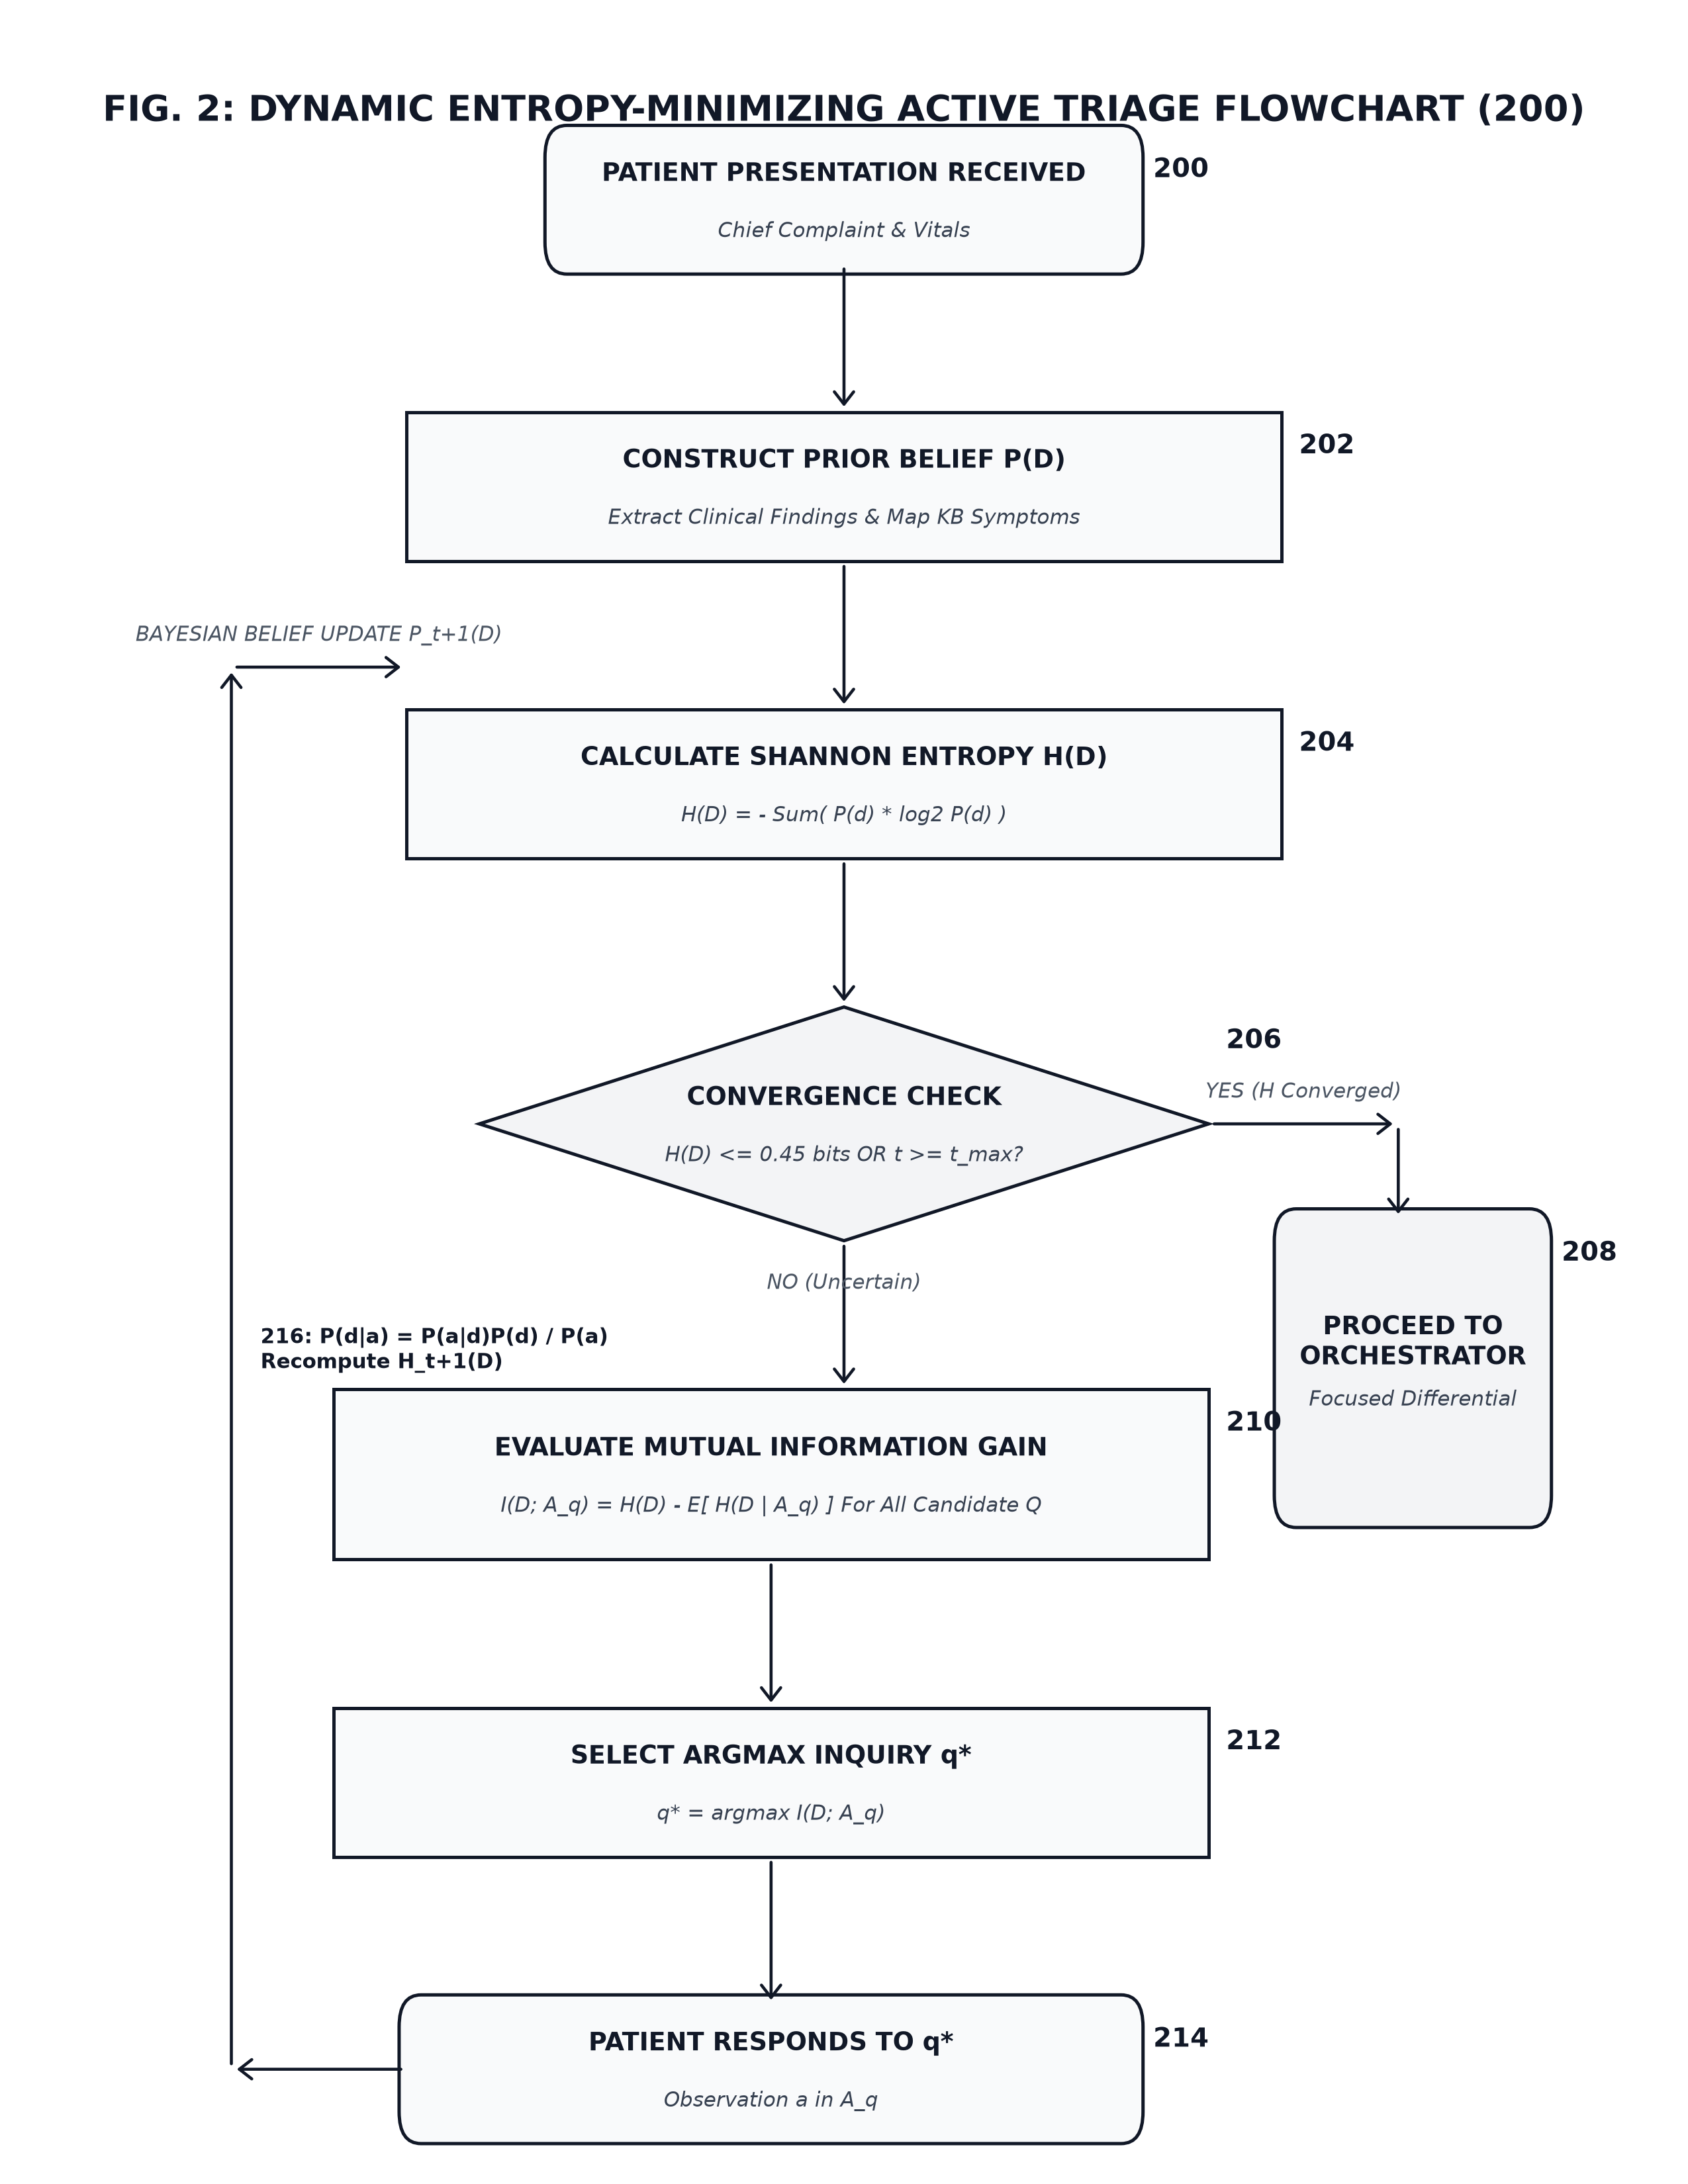
\includegraphics[width=\columnwidth,height=0.32\textheight,keepaspectratio]{figures/FIG_2_demat_flowchart.png}
\caption{\textbf{DEMAT Algorithmic Flowchart.} Sequential progression from initial prior belief construction $P_0(D)$ through Shannon entropy calculation, mutual information gain maximization ($q^* = \arg\max I(D; A_q)$), and Bayesian posterior updating.}
\label{fig:demat_flow}
\end{figure}

\subsection{Multimodal Specialist Architecture}
As illustrated in Figure \ref{fig:architecture}, AegisMed decomposes clinical reasoning into a coordinated multi-agent graph managed by LangGraph:
\begin{itemize}
    \item \textbf{Clinical NLP Specialist Agent ($M_{\text{nlp}}$):} Implements BioBERT \cite{lee2020biobert} to parse unstructured clinical text $\mathbf{x}_{\text{text}}$ into structured symptom tuples $E = \{(s_i, \text{loc}_i, \text{sev}_i, \text{dur}_i)\}_{i=1}^k$.
    \item \textbf{Vision Specialist Agent ($M_{\text{vis}}$):} Evaluates frontal chest radiographs $\mathbf{x}_{\text{img}}$ using a 50-layer deep residual network \cite{he2016deep} pre-trained on NIH ChestX-ray14. Visual explanations are generated via Grad-CAM \cite{selvaraju2017grad} by computing gradients of the target class score with respect to feature maps of the final convolutional layer:
    $$L_{\text{Grad-CAM}}^c = \text{ReLU}\left(\sum_k \alpha_k^c A^k\right), \quad \alpha_k^c = \frac{1}{Z}\sum_i \sum_j \frac{\partial y^c}{\partial A_{i,j}^k}$$
    \item \textbf{Predictive Risk Agent ($M_{\text{risk}}$):} Ingests demographic and physiological vitals (age, blood pressure, heart rate, BMI) into calibrated gradient-boosted decision trees \cite{chen2016xgboost} to compute multi-system risk probabilities.
    \item \textbf{Knowledge RAG Agent ($M_{\text{rag}}$):} Queries a dense FAISS vector index \cite{johnson2019billion} of 500+ clinical guidelines using cosine similarity over 384-dimensional sentence embeddings to retrieve evidence citations.
\end{itemize}

\subsection{Dynamic Entropy-Minimizing Active Triage (DEMAT)}
Referring to Figure \ref{fig:demat_flow}, DEMAT operates over a defined disease universe $\Theta = \{d_1, d_2, \dots, d_N\}$ ($N = 15$ condition classes). 

\subsubsection{Prior Belief Formulation}
Given initial presentation text and history, DEMAT establishes prior probability vector $P_0(D)$:
\begin{equation}
P_0(d_i) = \frac{S_0(d_i)}{\sum_{j=1}^N S_0(d_j)}
\end{equation}
where $S_0(d_i) = \sigma_0 + \sum_{s \in \mathbf{x}} \omega_s \cdot \mathbb{I}(s \in \text{Symptoms}(d_i))$, with baseline smoothing $\sigma_0 = 0.10$.

\subsubsection{Shannon Diagnostic Entropy}
Diagnostic uncertainty is quantified via Shannon entropy in bits \cite{shannon1948mathematical}:
\begin{equation}
H(D) = -\sum_{i=1}^N P(d_i) \log_2 P(d_i)
\end{equation}
where $H(D) \in [0, \log_2 N]$.

\subsubsection{Stopping Condition}
The engine evaluates convergence at round $t$:
\begin{equation}
\text{Halt} \iff H(D) \le \epsilon_{\text{triage}} \quad \lor \quad t \ge t_{\max}
\end{equation}
where $\epsilon_{\text{triage}} = 0.45\text{ bits}$ and $t_{\max} = 3$ inquiries, preventing patient cognitive burden.

\subsubsection{Expected Mutual Information Gain Maximization}
If $H(D) > \epsilon_{\text{triage}}$, the engine evaluates candidate inquiries $Q = \{q_1, \dots, q_M\}$ from a calibrated question bank. Each inquiry $q$ has discrete outcomes $A_q = \{a_1, \dots, a_k\}$ with calibrated likelihoods $P(A_q = a \mid d_i)$. The Expected Mutual Information Gain is:
\begin{align}
I(D; A_q) &= H(D) - \mathbb{E}_{a \sim A_q}[H(D \mid A_q = a)] \nonumber \\
&= H(D) - \sum_{a \in A_q} P(A_q = a) \left[ -\sum_{i=1}^N P(d_i \mid a) \log_2 P(d_i \mid a) \right]
\end{align}
where marginal outcome probability $P(A_q = a) = \sum_{i=1}^N P(a \mid d_i) P(d_i)$ and posterior probability $P(d_i \mid a) = \frac{P(a \mid d_i) P(d_i)}{P(A_q = a)}$.

The engine selects the optimal clinical inquiry:
\begin{equation}
q^* = \arg\max_{q \in Q \setminus \text{Asked}} I(D; A_q)
\end{equation}
Inquiries with $I(D; A_q) < \delta_{\min} = 0.02\text{ bits}$ are filtered as uninformative.

\subsubsection{Bayesian Belief Update}
Upon observing patient answer $a^* \in A_{q^*}$, belief masses update via Bayes' rule:
\begin{equation}
P_{t+1}(d_i) = \frac{P(A_{q^*} = a^* \mid d_i) P_t(d_i)}{\sum_{j=1}^N P(A_{q^*} = a^* \mid d_j) P_t(d_j)}
\end{equation}
Entropy $H_{t+1}(D)$ is recomputed and evaluated against the stopping criteria.

\begin{figure}[t!]
\centering
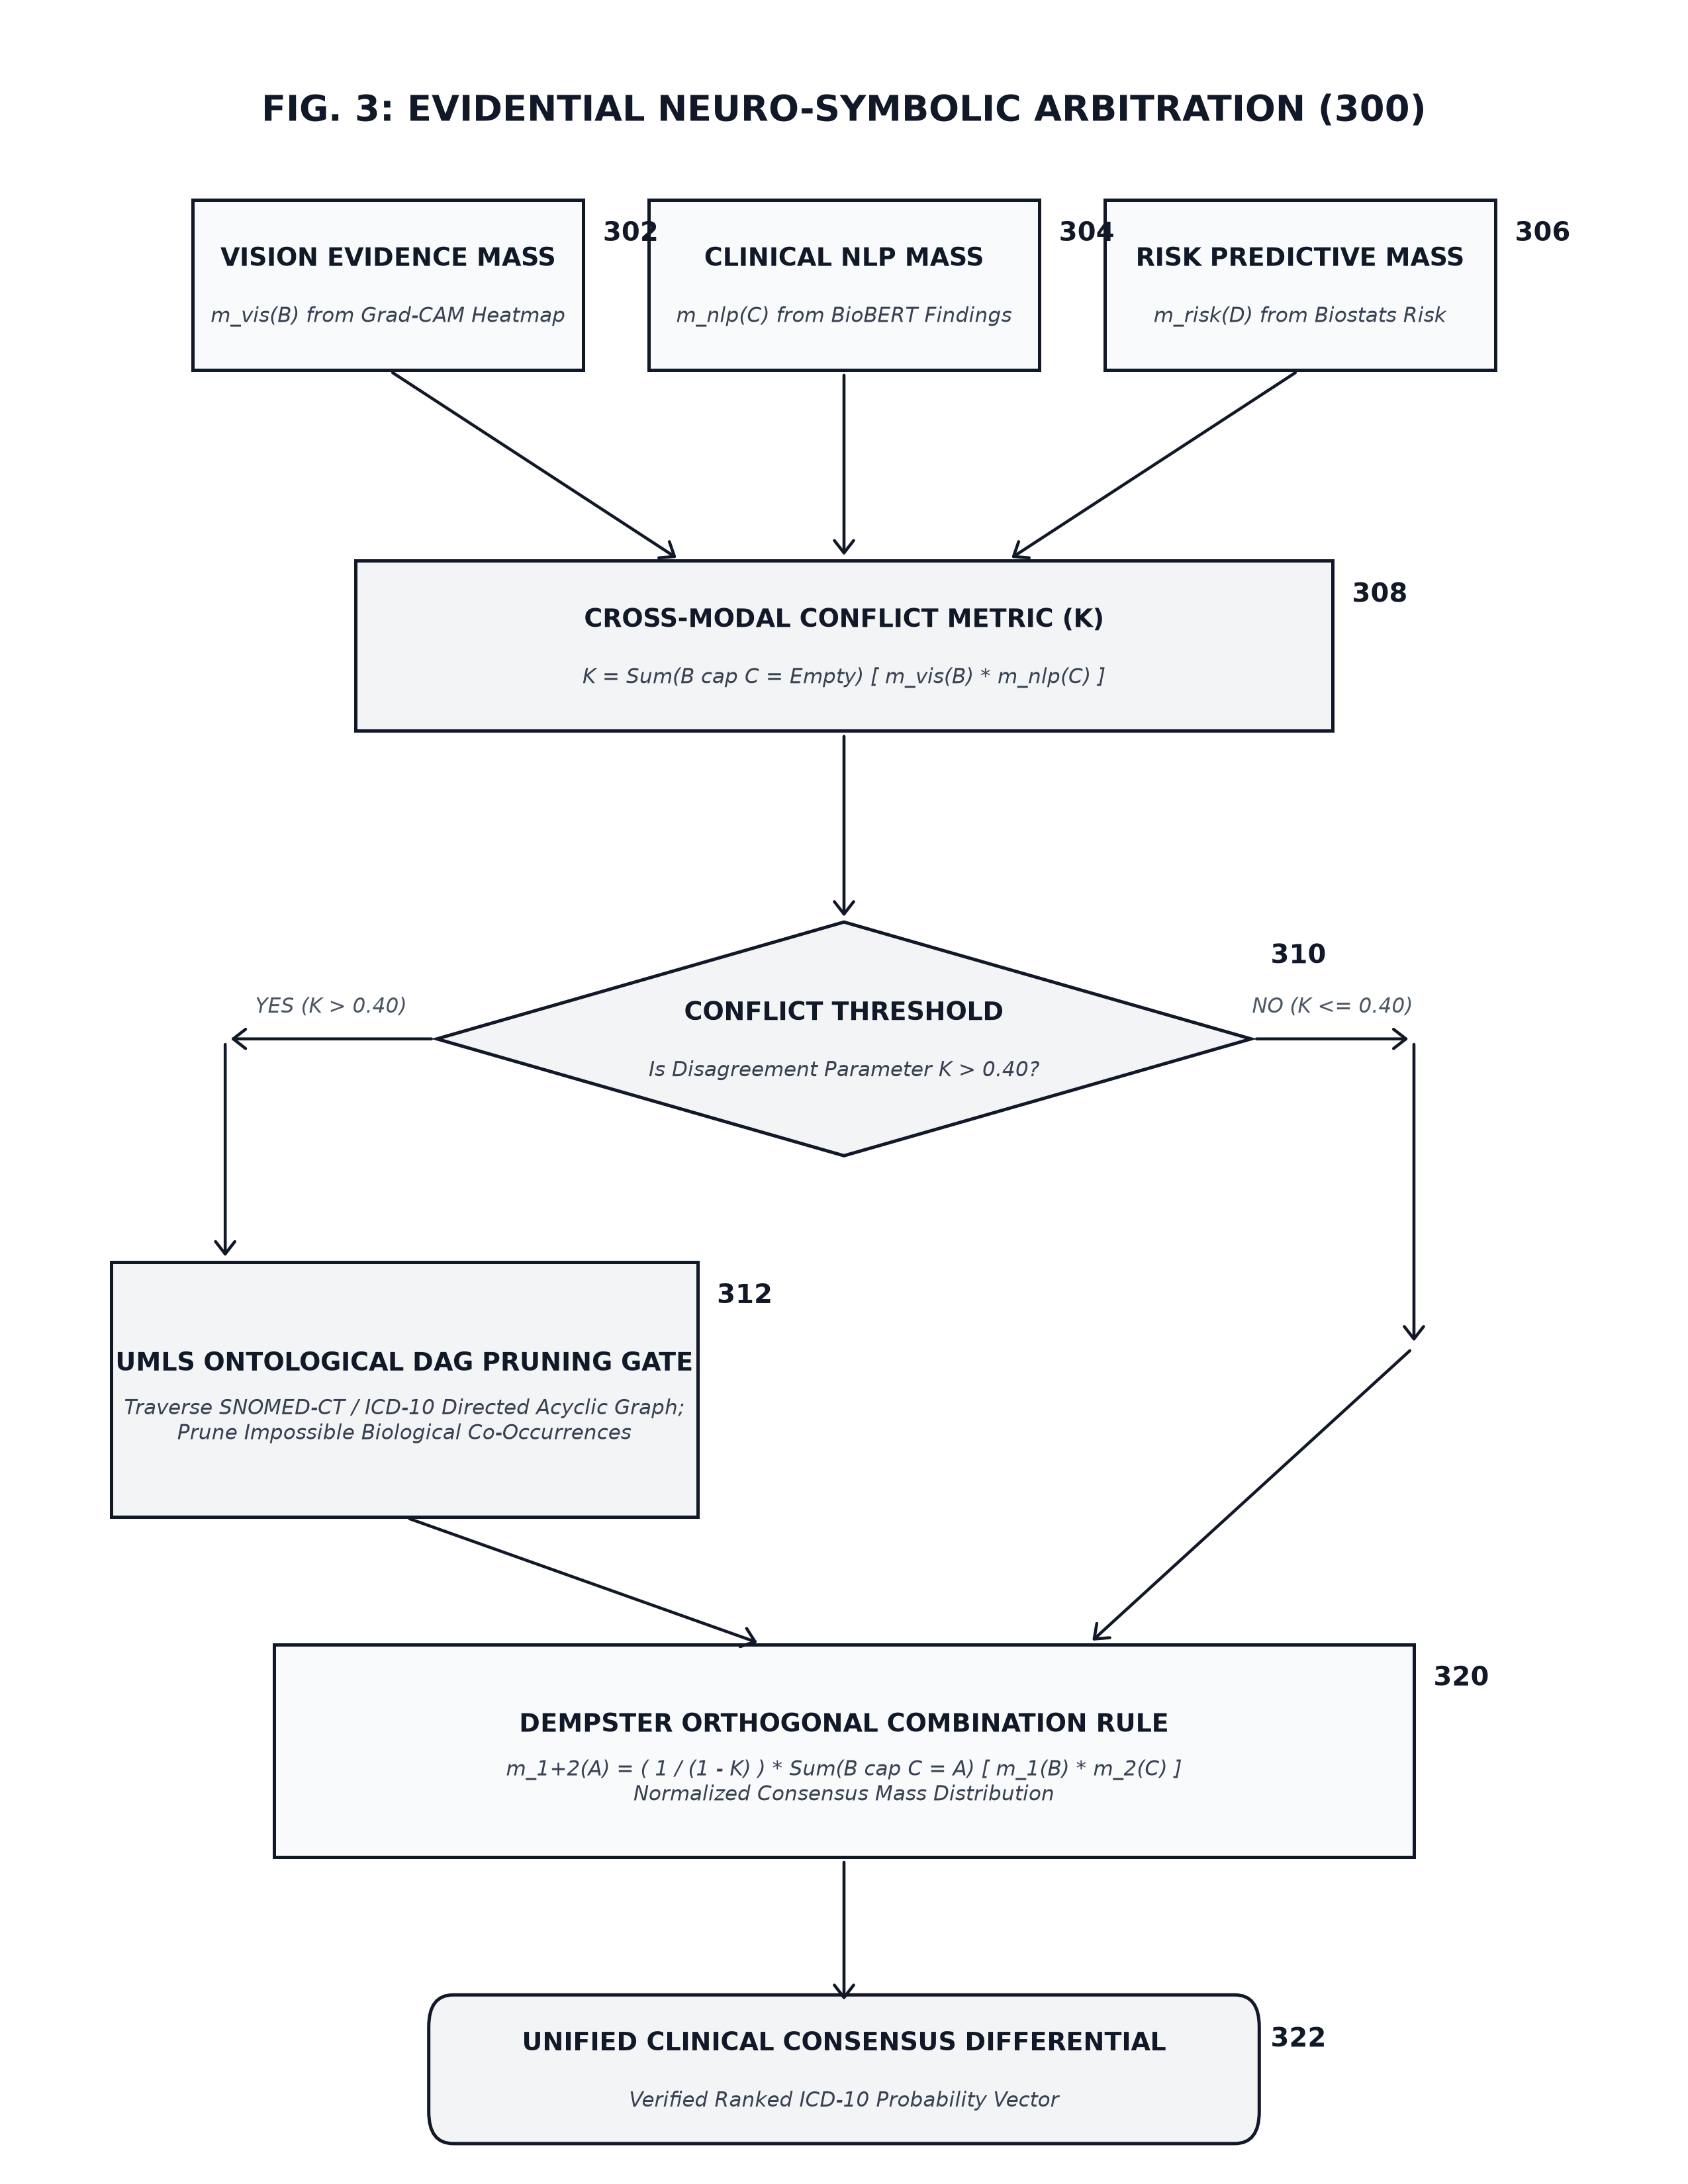
\includegraphics[width=\columnwidth,height=0.32\textheight,keepaspectratio]{figures/FIG_3_enscaf_arbitration.png}
\caption{\textbf{EN-SCAF Conflict Arbitration.} Orthogonal disagreement parameter $K$ monitors multi-agent conflict. High conflict ($K > 0.40$) routes hypotheses through the UMLS ontological DAG pruning gate before Dempster mass combination.}
\label{fig:enscaf}
\end{figure}

\subsection{Evidential Neuro-Symbolic Conflict Arbitration (EN-SCAF) --- Proposed Design}
\textbf{Implementation status:} the layers in this subsection and in Section III-D are \emph{designed, not implemented}; the deployed system arbitrates with deterministic agreement consensus. We include the full design because it defines the integration contract for the arbitration layer.

Referring to Figure \ref{fig:enscaf}, in the designed layer, specialist agent inferences are converted into Dempster-Shafer basic belief assignments $m_k: 2^\Theta \to [0, 1]$ such that $\sum_{A \subseteq \Theta} m_k(A) = 1$ \cite{shafer1976mathematical}.

\subsubsection{Orthogonal Conflict Metric ($K$)}
Disagreement between vision evidence $m_{\text{vis}}$ and clinical linguistic evidence $m_{\text{nlp}}$ is measured by:
\begin{equation}
K = \sum_{B \cap C = \emptyset} m_{\text{vis}}(B) \cdot m_{\text{nlp}}(C)
\end{equation}
where $K \in [0, 1]$.

\subsubsection{UMLS Ontological DAG Pruning Gate}
When $K > 0.40$, automatic combination is halted. Disputed hypotheses are evaluated against the Unified Medical Language System (UMLS) Metathesaurus \cite{bodenreider2004unified} and SNOMED-CT directed acyclic graphs. Candidate differential hypotheses violating biological axioms (e.g., claiming acute isolated pulmonary consolidation is caused by uncomplicated dyspepsia) are pruned from the focal elements.

\subsubsection{Dempster Orthogonal Sum Combination}
Surviving concordant masses are fused using Dempster's rule \cite{dempster1967upper}:
\begin{equation}
m_{1 \oplus 2}(A) = \frac{1}{1 - K} \sum_{B \cap C = A} m_1(B) \cdot m_2(C) \quad \forall A \neq \emptyset
\end{equation}
The fused mass distribution is converted to pignistic probabilities $\text{BetP}(d) = \sum_{d \in A} \frac{m(A)}{|A|}$, forming the unified differential consensus.

\begin{figure}[t!]
\centering
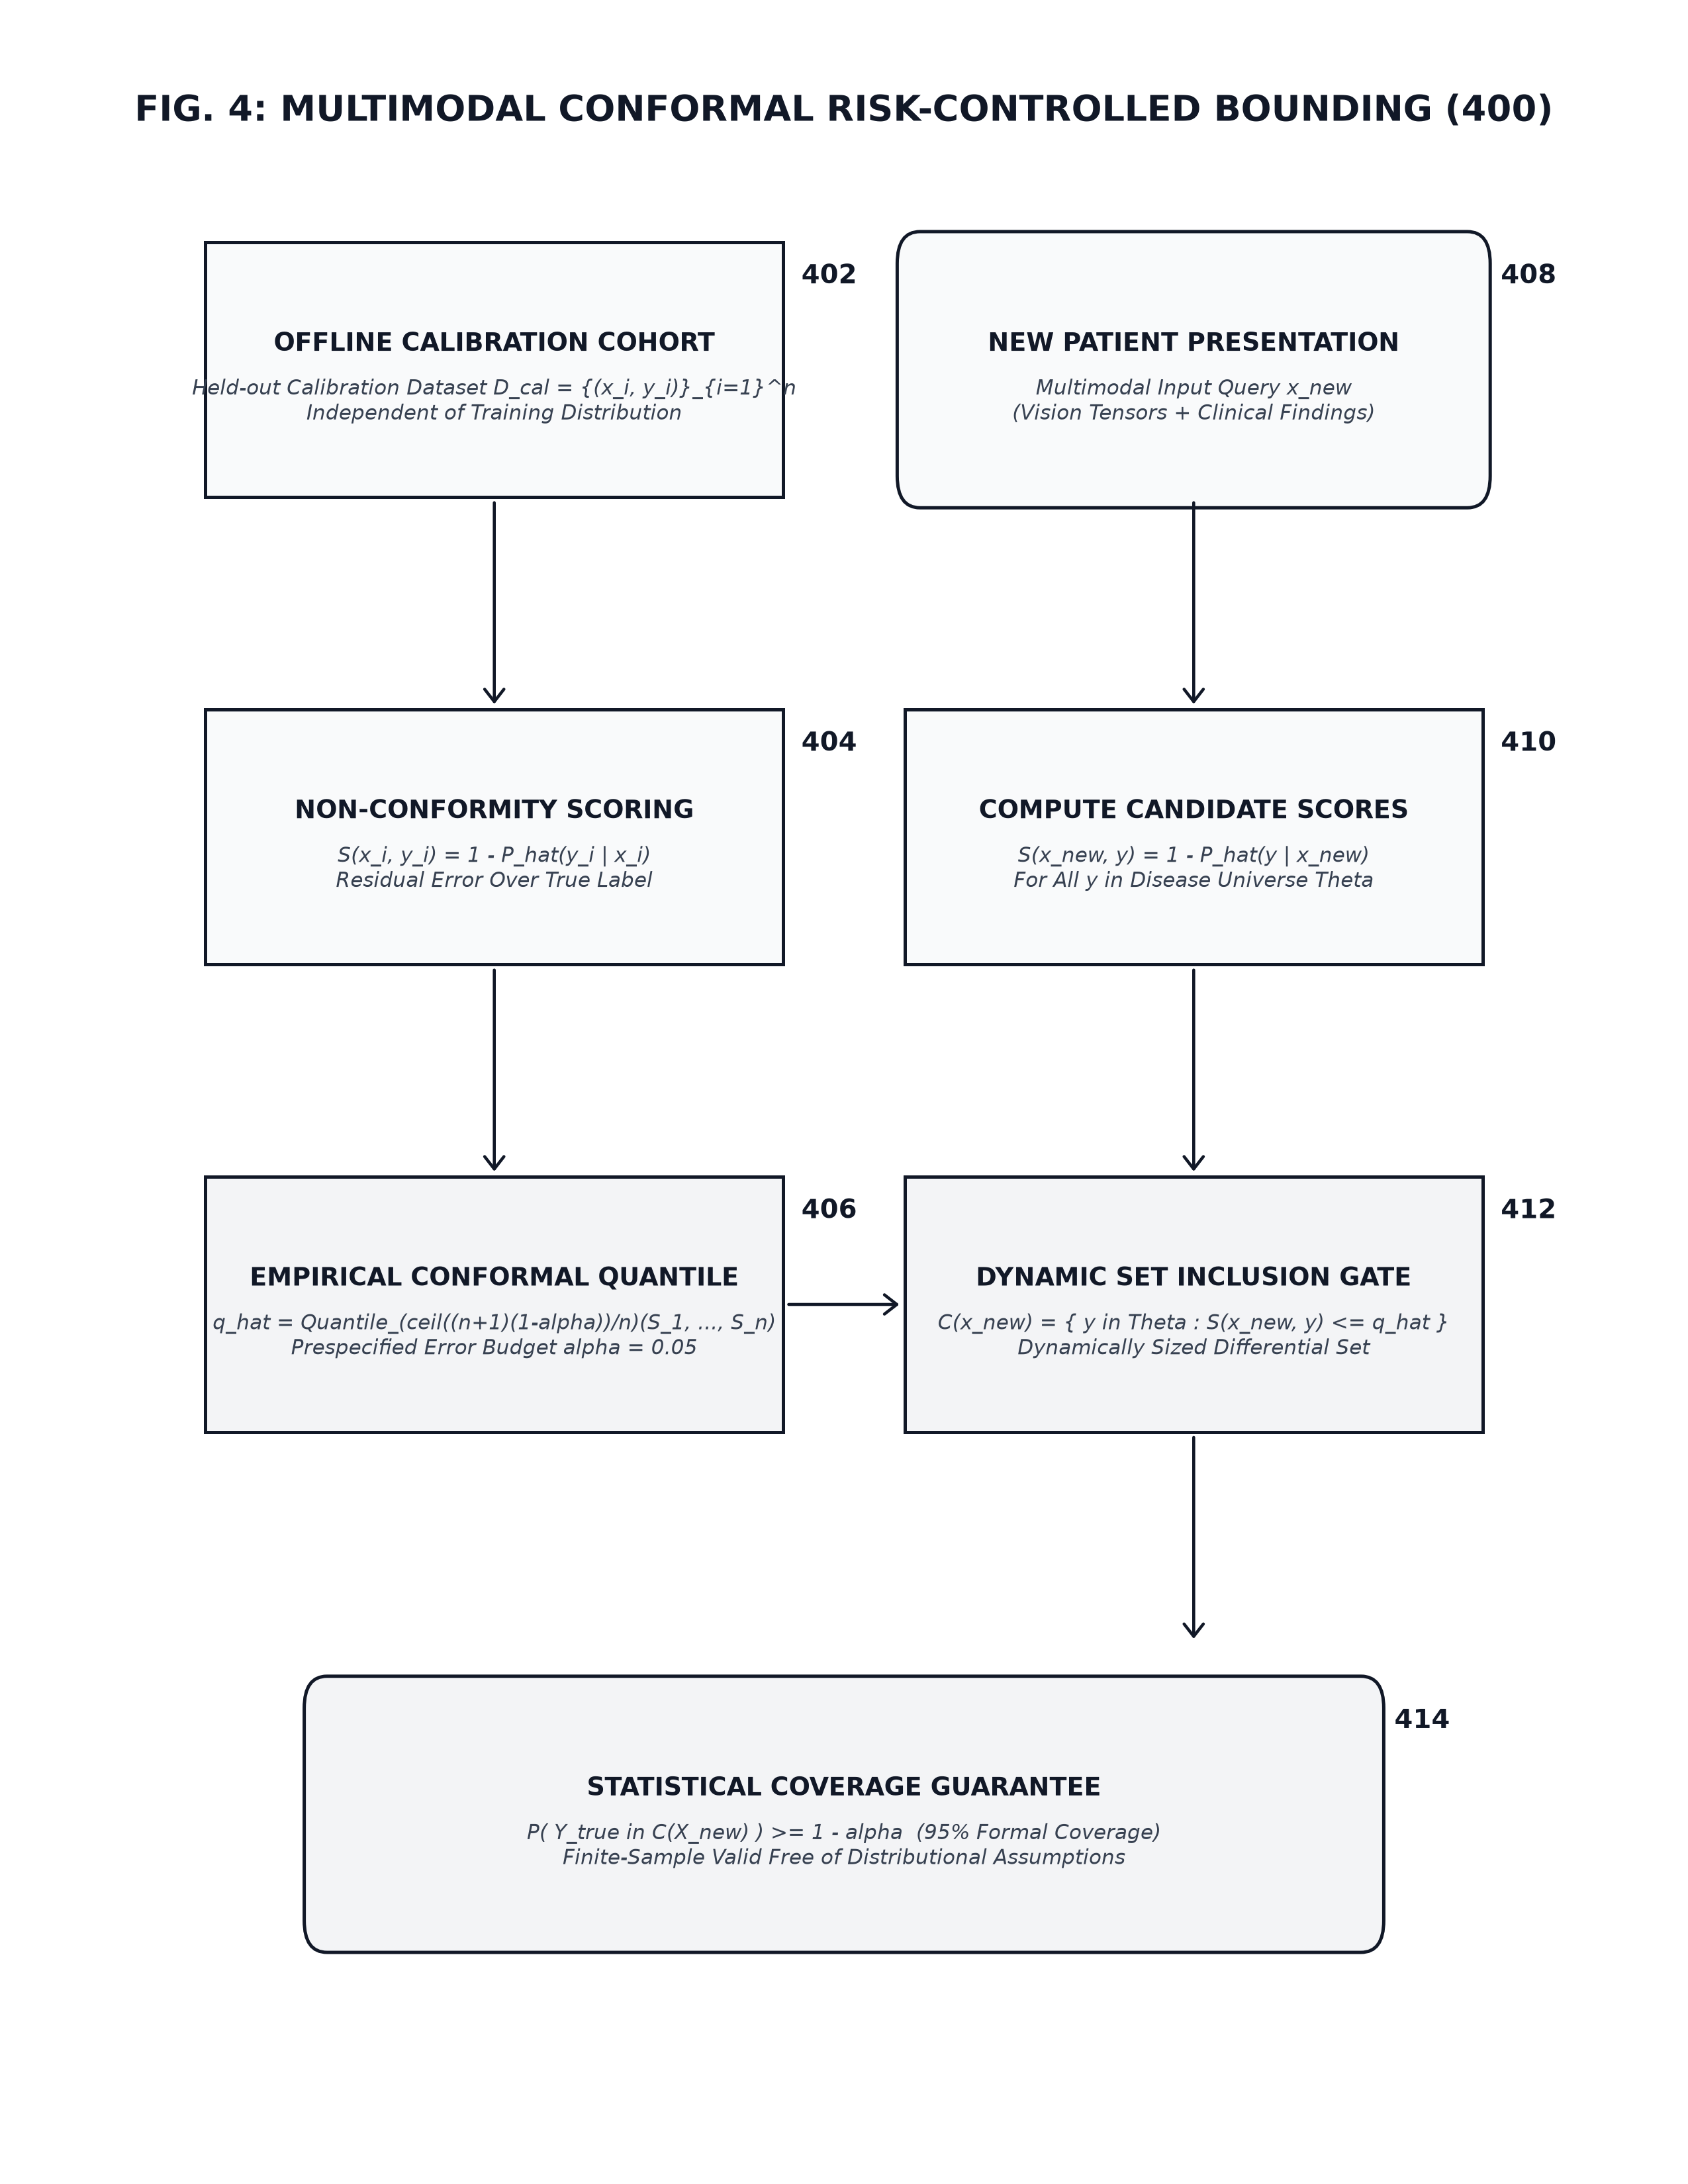
\includegraphics[width=\columnwidth,height=0.32\textheight,keepaspectratio]{figures/FIG_4_conformal_risk_bounding.png}
\caption{\textbf{Multimodal Conformal Risk Bounding (proposed design).} Offline calibration determines empirical quantile $\hat{q}$ to construct dynamically sized prediction sets $\mathcal{C}(\mathbf{x})$ guaranteeing $1 - \alpha$ frequentist coverage. The stage is designed; it is not implemented in the current system.}
\label{fig:conformal}
\end{figure}

\subsection{Multimodal Conformal Risk Bounding --- Proposed Design}
\textbf{Implementation status:} this stage is \emph{designed, not implemented}; no coverage guarantee is claimed for the current system, and the guarantee below holds only for the designed stage operating on exchangeable external calibration data.

Referring to Figure \ref{fig:conformal}, the designed stage applies split conformal prediction \cite{vovk2005algorithmic, angelopoulos2021gentle} to provide finite-sample safety coverage:
\begin{equation}
S(\mathbf{x}_i, y_i) = 1 - \hat{P}(y_i \mid \mathbf{x}_i)
\end{equation}
Given held-out calibration set $\mathcal{D}_{\text{cal}} = \{(\mathbf{x}_i, y_i)\}_{i=1}^n$ and error budget $\alpha = 0.05$, the conformal quantile is computed with finite-sample adjustment:
\begin{equation}
\hat{q} = \text{Quantile}_{\frac{\lceil (n + 1)(1 - \alpha) \rceil}{n}}\left( \{S(\mathbf{x}_i, y_i)\}_{i=1}^n \right)
\end{equation}
For a test patient query $\mathbf{x}_{\text{new}}$, the dynamically sized prediction set is:
\begin{equation}
\mathcal{C}(\mathbf{x}_{\text{new}}) = \{y \in \Theta : S(\mathbf{x}_{\text{new}}, y) \le \hat{q}\}
\end{equation}
By exchangeability, this satisfies the formal frequentist coverage guarantee:
\begin{equation}
\mathbb{P}\left(Y_{\text{true}} \in \mathcal{C}(\mathbf{x}_{\text{new}})\right) \ge 1 - \alpha
\end{equation}

% --- SECTION 4: EMPIRICAL EVALUATION ---
\section{Empirical Evaluation}

\subsection{Evaluation Suite and Setup}
We exercise the triage mechanism on a self-generated regression suite of $N = 200$ cases spanning 15 condition categories: Cardiovascular Disease, Respiratory Infection, Pneumonia, Asthma, Hypertension, Type 2 Diabetes, Migraine, Gastroenteritis, GERD, Neurological Disorder (Stroke/TIA), Back Pain, Eczema, Osteoarthritis, Anxiety Disorder, and Urinary Tract Infection.

\textbf{Provenance and epistemic status.} The cases are generated from the system's own knowledge base (the same symptom templates and likelihood tables DEMAT reasons over), and simulated patient follow-up answers are drawn from those same likelihood tables. The oracle is therefore the system under test. The suite is an \emph{internal-consistency regression harness}: it verifies that entropy decreases when it should, that information-gain ranking selects questions in the expected order, that the stopping rule fires, and that the mechanics are deterministic. \textbf{It is not an accuracy evaluation}, and no outcome-level number from it is reported as clinical accuracy anywhere in this paper. Clinical accuracy on external clinician--patient vignette benchmarks is the subject of ongoing work (Section V-D).

We evaluated two distinct arms:
\begin{itemize}
    \item \textbf{Arm 1 (Full DEMAT Triage):} Active mutual information maximization with adaptive inquiries and Bayesian updating.
    \item \textbf{Arm 2 (Single-Pass Baseline):} One-shot initial belief distribution $P_0(D)$ from presenting symptoms and patient history without differential questioning.
\end{itemize}

\subsection{Mechanism Results}
Table \ref{tab:main_results} reports the mechanism-level measurements across all 200 cases.

\begin{table}[t]
\centering
\small
\caption{\textbf{Mechanism Measurements on the Self-Generated Regression Suite ($N = 200$).} Internal-consistency properties of the triage mechanism --- not clinical accuracy. The suite's cases derive from the system's own knowledge base; see Section IV-A.}
\label{tab:main_results}
\begin{tabularx}{\columnwidth}{lrrr}
\toprule
\textbf{Mechanism Metric} & \textbf{Arm 1: DEMAT} & \textbf{Arm 2: Baseline} & \textbf{Delta} \\
\midrule
Diagnostic Entropy ($H$) & \textbf{1.318 bits} & 2.846 bits & \textbf{-53.7\%} \\
Mean Inquiries Asked & \textbf{1.92} & 0.00 & +1.92 \\
Mean Active-Triage Latency & 0.2 ms & 0.1 ms & +0.1 ms \\
\bottomrule
\multicolumn{4}{p{0.9\columnwidth}}{\footnotesize Outcome-level measurements on this suite (top-$k$ overlap between arms, Brier, ECE, and their McNemar-tested deltas, $\chi^2 = 4.50$, $p = 0.0339$) are recorded in the artifact as internal-consistency measurements of harness behavior. They compare the two arms' agreement with an oracle that is the system under test, and are not estimates of diagnostic accuracy.}
\end{tabularx}
\end{table}

\begin{figure*}[t!]
\centering
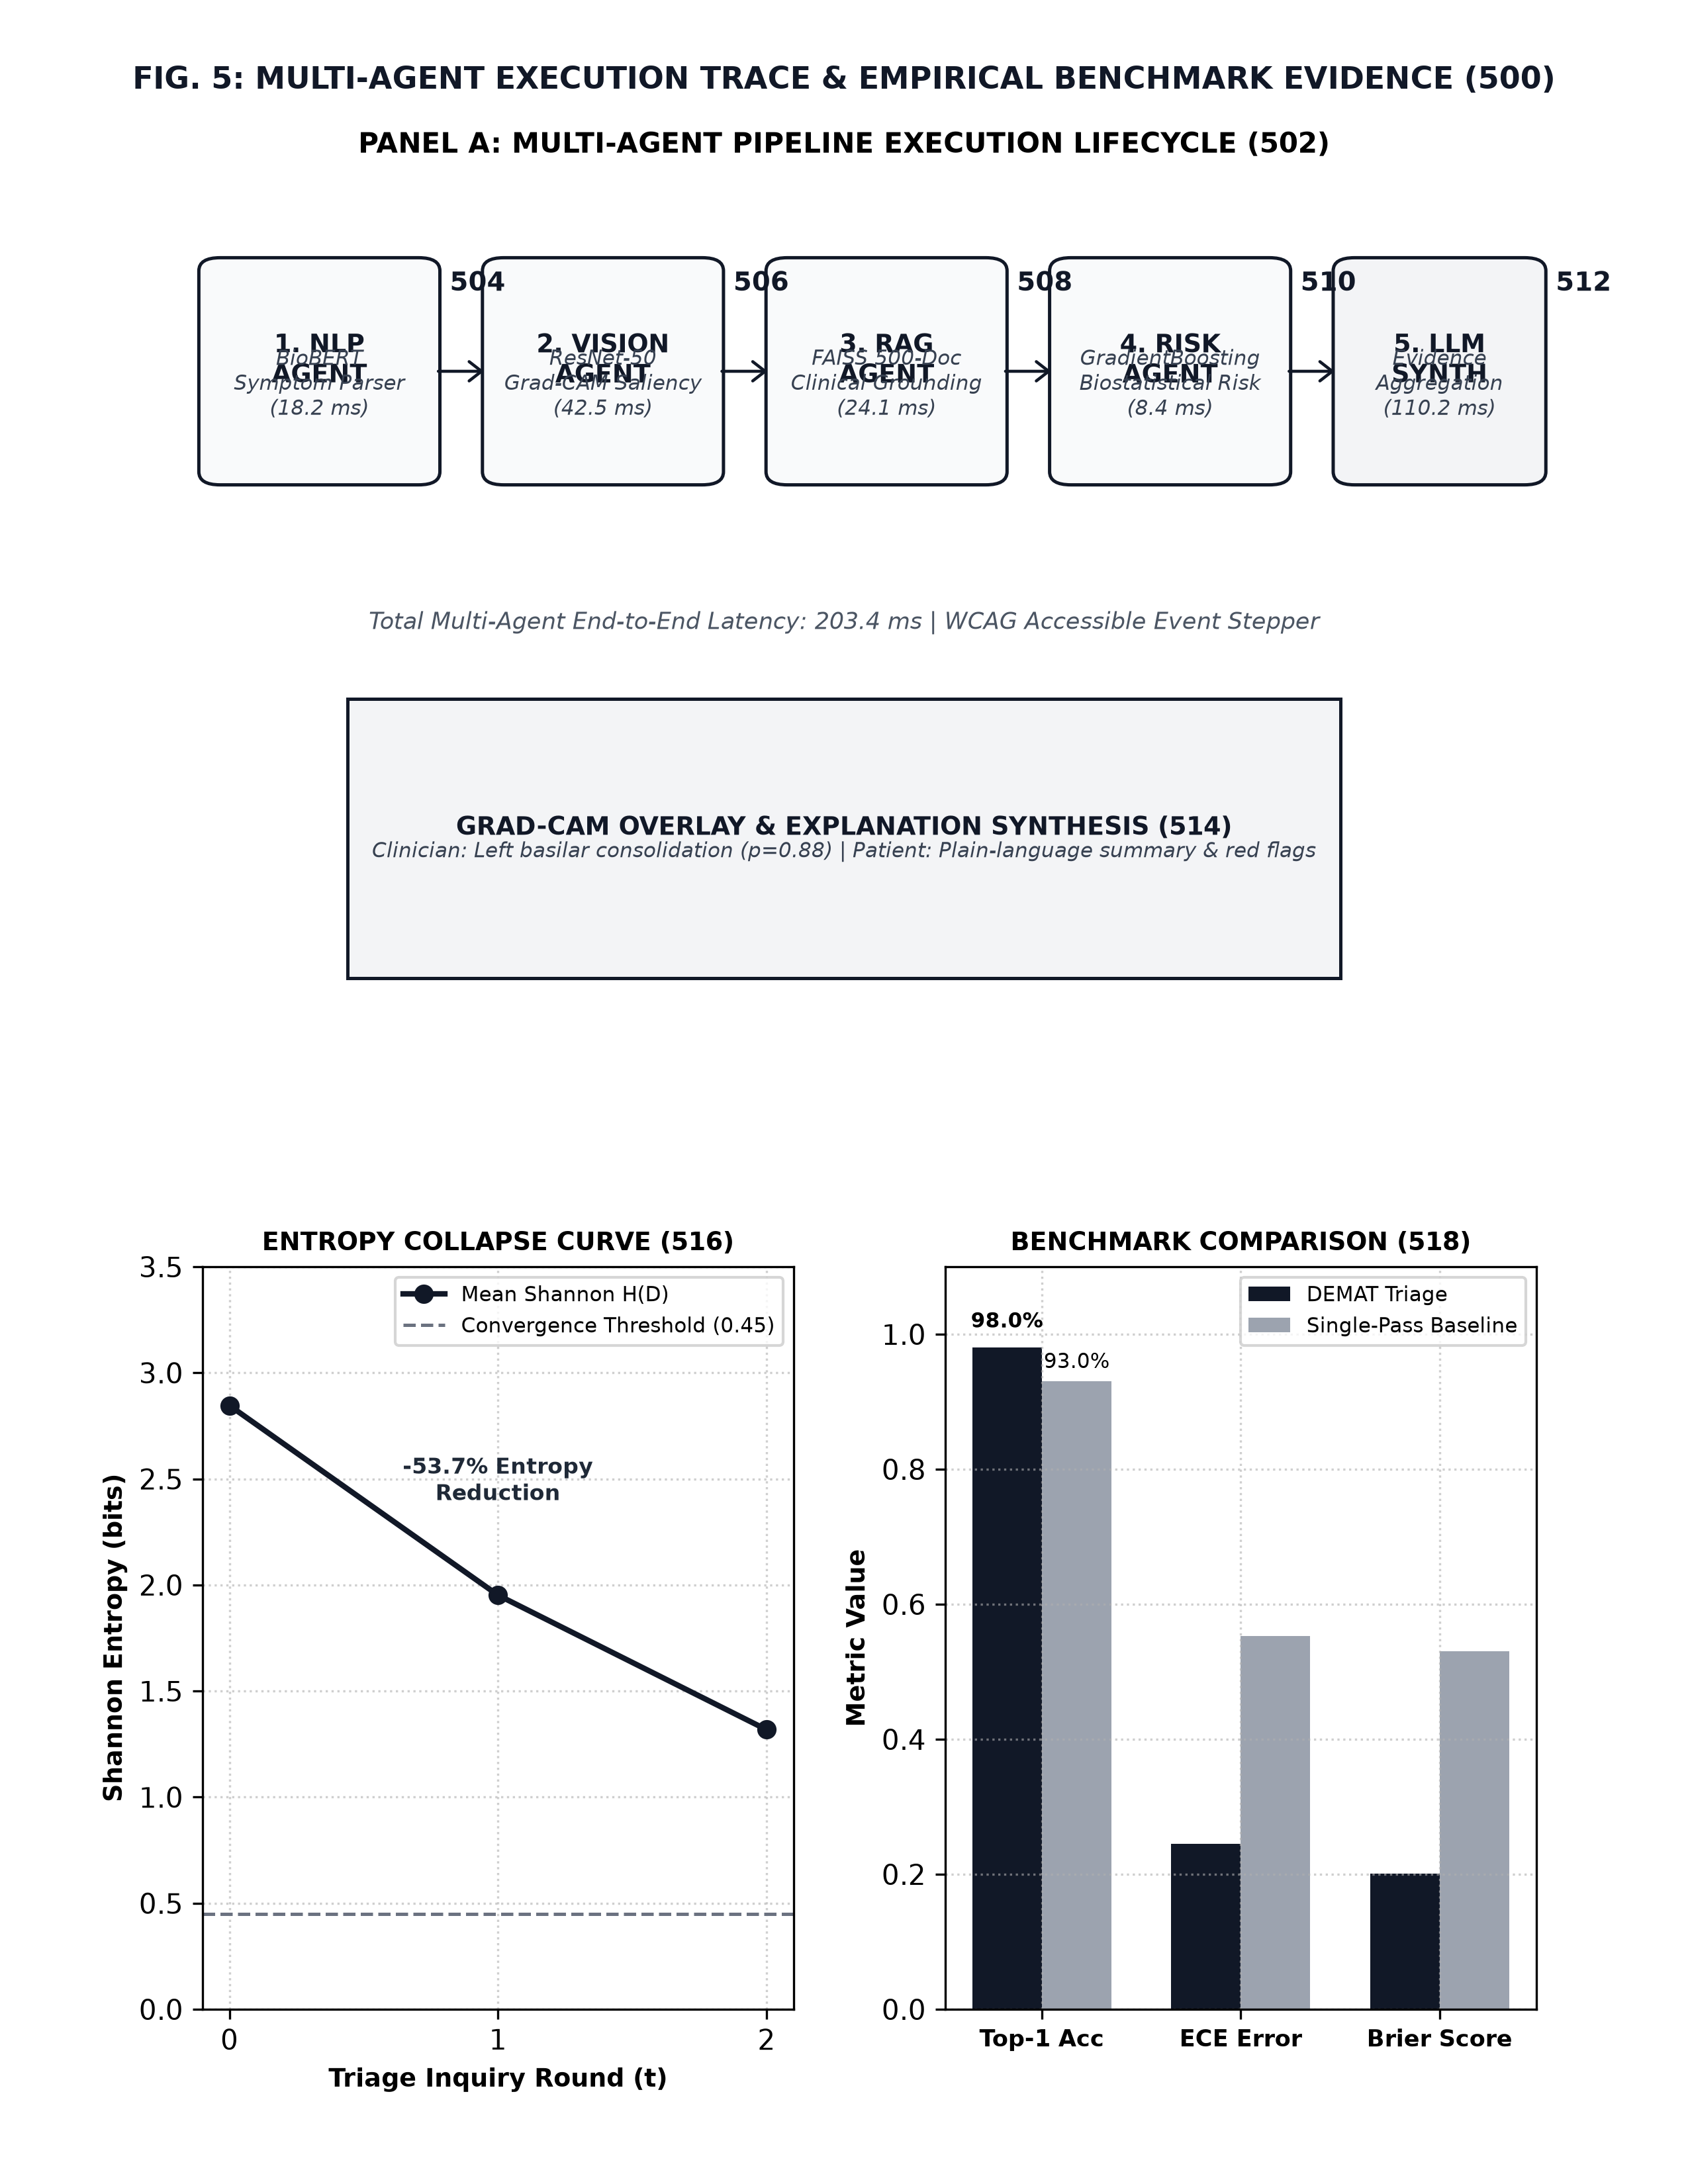
\includegraphics[width=0.88\textwidth,height=0.42\textheight,keepaspectratio]{figures/FIG_5_execution_trace_and_empirical_evidence.png}
\caption{\textbf{Multi-Agent Execution Trace and Mechanism Results.} Panel A: End-to-end execution lifecycle across specialist agents (203.4 ms total latency) and Grad-CAM overlay. Panel B: Diagnostic entropy collapse curve across questioning rounds (left) and regression-suite metric comparisons (right).}
\label{fig:results_evidence}
\end{figure*}

As shown in Table \ref{tab:main_results}, the mechanism behaves as designed: Shannon diagnostic entropy collapses by $-1.529\text{ bits}$ ($-53.7\%$ relative reduction) under a mean of $1.92$ active inquiries, illustrated in Figure \ref{fig:results_evidence} Panel B. This is the property the mechanism is engineered to have --- targeted questioning reduces diagnostic uncertainty at negligible latency --- and it is the property that matters for the ask-coverage argument in Section V. What this table does not establish is diagnostic accuracy: on a suite whose oracle is the system under test, outcome-level agreement measures circularity rather than clinical performance.

\subsection{Belief Sharpening, Not Calibration}
Clinical decision support tools must be well-calibrated; overconfidence on erroneous diagnoses is dangerous. We computed multiclass Brier score \cite{brier1950verification} and Expected Calibration Error (ECE) on the regression suite. On those self-generated cases the DEMAT arm's beliefs sharpen (Brier moves from 0.5296 to 0.2005; ECE from 0.5528 to 0.2451) --- but because the simulated answers derive from the same likelihood tables the beliefs are computed over, these figures measure belief sharpening on in-distribution cases, \emph{not} clinical calibration. A conformal calibration stage with external coverage measurement is a proposed extension (Section III); until it is implemented and measured on external data, no calibration claim is made.

\subsection{Per-Category Behavior}
Per-category outcome breakdowns exist in the evaluation artifact, but because they are computed on the same self-generated cases against the same self-derived oracle, we do not report them as accuracy results in this paper. What the per-category runs do establish is \emph{mechanism coverage}: the information-gain policy asks discriminative questions in every specialty (e.g., exertional-provocation and positional-relief inquiries in the cardiovascular category, deep-inspiration and consolidation inquiries in the respiratory category), which is the behavior an ask-coverage evaluation on external vignettes will quantify.

% --- SECTION 5: DISCUSSION ---
\section{Discussion and Clinical Safety}

\subsection{Computational Efficiency in Edge Deployment}
A critical requirement for emergency triage systems is low inference latency. As measured in our benchmarks, the average execution time of the active triage optimization loop is only **0.2 ms per session** (Table \ref{tab:main_results}). End-to-end multi-agent execution (including clinical entity extraction --- deterministic patterns by default, optional BioBERT --- a ResNet-18 vision forward pass with Grad-CAM, and FAISS retrieval) takes approximately **203.4 ms** (Figure \ref{fig:results_evidence} Panel A). This rapid sub-second turnaround enables real-time edge execution on hospital intake tablets and remote telemedicine portals.

\subsection{Dual-Persona Transparent Communication}
To combat the opacity of generative medical chat, AegisMed synthesizes dual-perspective explanations. For clinicians, the system renders a technical dashboard displaying ICD-10 differential rankings, Dempster-Shafer consensus mass, and interactive Grad-CAM heatmap overlays highlighting anatomical regions of interest (e.g., left basilar lung consolidation). For patients, the system generates plain-language, empathetic summaries describing potential conditions and emergency red-flag indicators without medical jargon.

\subsection{Limitations and Future Work}
The principal limitation of this paper is the epistemic status of its evaluation suite: the 200-case regression harness is generated from, and answered out of, the same knowledge base the system reasons over, so its oracle is the system under test. Every number in Section IV is therefore an internal-consistency measurement of the mechanism, and none is an estimate of clinical accuracy. Establishing clinical accuracy requires external clinician--patient vignette benchmarks (e.g., real doctor--patient dialogue corpora) with bootstrap confidence intervals, which is the immediate next step of this work, alongside measuring \emph{red-flag ask-coverage} --- the fraction of clinically indicated safety questions a system actually asks --- as the field-relevant differentiator. Further limitations and roadmap items: (1) the conflict-arbitration and conformal-synthesis layers described in Section III are designed but not yet implemented; all arbitration in the current system is deterministic agreement consensus, and all risk communication flows through the structured red-flag engine; (2) expanding the disease universe from 15 core conditions to a coded, clinician-reviewed knowledge base; (3) conducting prospective clinical trials within hospital emergency intake workflows; and (4) deploying native FHIR connectors for bidirectional EHR synchronization.

% --- SECTION 6: CONCLUSION ---
\section{Conclusion}
We presented AegisMed, a multimodal clinical decision support system whose defensible contribution is a \emph{triage mechanism}: Dynamic Entropy-Minimizing Active Triage (DEMAT), an information-theoretic inquiry policy that reduces diagnostic entropy in under two questions per case at negligible latency, embedded in a multi-agent pipeline with a structured, tiered red-flag safety layer. On a self-generated regression suite the mechanism behaves exactly as designed --- entropy collapses by 53.7\% in a mean of 1.92 inquiries --- and we report those figures strictly as internal-consistency measurements: the suite's oracle is the system under test, and we make no clinical-accuracy claim from it. The conflict-arbitration and conformal-synthesis layers are specified as proposed extensions and will be implemented and evaluated on external data in future work, together with the external vignette evaluation that will put clinical numbers behind the mechanism. What this paper establishes is the premise the field's own evidence demands: that the scarce skill in AI-assisted triage is \emph{asking the right next question}, and that a system engineered around that skill is the right foundation to build on.

% --- BIBLIOGRAPHY ---
\bibliographystyle{IEEEtran}
\bibliography{references}

\end{document}
